\title{DPIoT - Riassunto}
\author{
	Tommaso Puccetti \\
	Studente presso Universita degli studi di Firenze
}
\date{\today}
\documentclass[12pt]{article}
\usepackage[english]{babel}
\usepackage{graphicx}
\usepackage{hyperref}
\usepackage[procnames]{listings}
\usepackage{color}


\definecolor{keywords}{RGB}{255,0,90}
\definecolor{comments}{RGB}{0,0,113}
\definecolor{red}{RGB}{160,0,0}
\definecolor{green}{RGB}{0,150,0}

\lstset{language=Python, 
	backgroundcolor=\color{white},
	basicstyle=\ttfamily\small, 
	keywordstyle=\color{keywords},
	commentstyle=\color{comments},
	stringstyle=\color{green},
	showstringspaces=false,
	identifierstyle=\color{black},
	procnamekeys={def,class},
}


\begin{document}
	\maketitle
	\tableofcontents
	\listoftables
	\listoffigures
	
\section{Communication Mechanisms}
	
	\subsection{Basi}
	
		\subsubsection{Middleware}
				
			\begin{figure}[h!]
				\centering
				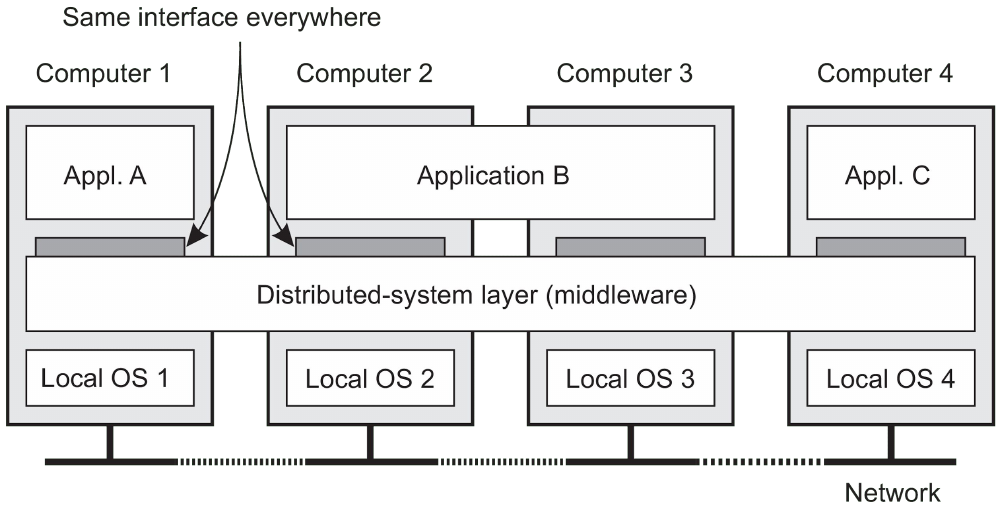
\includegraphics[scale=0.50]{img/middle.png}
				\caption{Livello Middleware}
			\end{figure}
			Il \textbf{middleware} è un insieme di applicazioni e protocolli "\textbf{general purpose}" che risiedono all'interno del livello applicativo. è dunque un livello software che astrae dall'eterogeneità di rete, hardware, sistemi operativi e linguaggi di programmazione, con lo \textbf{scopo di fornire interfacce comuni che assicurino  modelli di comunicazione e di computazione uniformi}.  Questo livello, dunque, costituisce un insieme di protocolli condivisi dalle applicazioni più specifiche al livello soprastante.
			In sintesi, un livello middleware offre servizi alle applicazioni quali:
			\begin{itemize}
				\item Comunicazione;
				\item Meccanismi di sicurezza;
				\item Transazioni
				\item Error-recovery;
				\item Gestione di risorse condivise.
			\end{itemize}
			\textbf{Questi servizi sono indipendenti rispetto alle specifiche applicazioni.} 
			Alcuni esempi:
			\begin{itemize}
				\item Protocolli di autenticazione e autorizzazione (criptografia ssh)
				\item Protocolli di commit. Sono utilizzati per realizzare l'atomicità nelle transazioni. Stabiliscono se in un insieme di processi tutti hanno svolto una particolare operazione o se non è stata svolta affatto.
			\end{itemize}
			Nello specifico vedremo come i \textbf{protocolli di comunicazione middleware supportino servizi di comunicazione ad alto livello} e permettano, per esempio, la chiamata a procedure o oggetti remoti in modo \textbf{trasparente.}
			 
		\subsubsection{Coordinazione diretta}	
			Un tipi di comunicazione nella quale le componenti partecipanti sono:
			\begin{itemize}
				\item \textbf{Referentially coupled}: durante la comunicazione gli attori utilizzano riferimenti espliciti ai loro interlocutori.
				\item \textbf{Temporally coupled}: entrambe le componenti devono essere in esecuzione (up and running).	
			\end{itemize}
			Il libro propone un'introduzione ai tipi di comunicazione (persist, transient, synchronous, asynchronous).
	\subsection{Remote Procedure Call}
		Molti sistemi distribuiti sono basati sullo scambio di messaggi tra processi, tuttavia questo tipo di approccio non permette di nascondere la comunicazione tra le componenti in modo da rendere trasparente il contesto distribuito. \\
		Una soluzione al problema è stata proposta da Nelson e Birrell (1984) introducendo una modalità completamente differente nella gestione della comunicazione nel contesto di un sistema distribuito.
		In breve la proposta è quella di chiamare procedure che sono localizzate su macchine remote:
		\begin{enumerate}
			\item quando A chiama B il processo chiamante in A è sospeso;
			\item l'esecuzione della procedura chiamata ha luogo in B;
			\item A invia i parametri della chiamata a B che a sua volta risponderà con il risultato della chiamata;
			\item \textbf{Nessun passaggio di messaggi è visibile dal punto di vista del programmatore.}
		\end{enumerate}
		La soluzione ha le seguenti problematiche:
		\begin{itemize}
			\item le procedure chiamante e chiamato si trovano su macchine diverse e non condividono lo stesso address space;
			\item la rappresentazione dei parametri e del risultato di ritorno può differire sulle macchine interessate;
			\item Le due macchine potrebbero crashare.
		\end{itemize}
		\begin{figure}[h!]
			\centering
			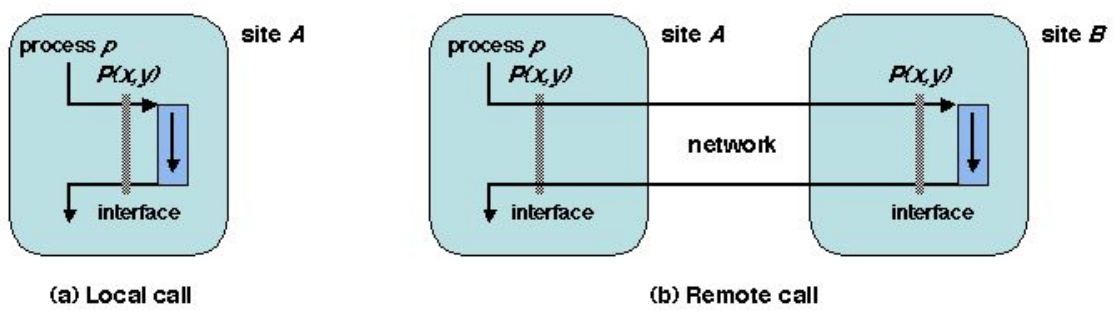
\includegraphics[scale=0.50]{img/proc.png}
			\caption{Chiamata a procedura locale vs remota}
		\end{figure}
		\begin{figure}[h!]
			\centering
			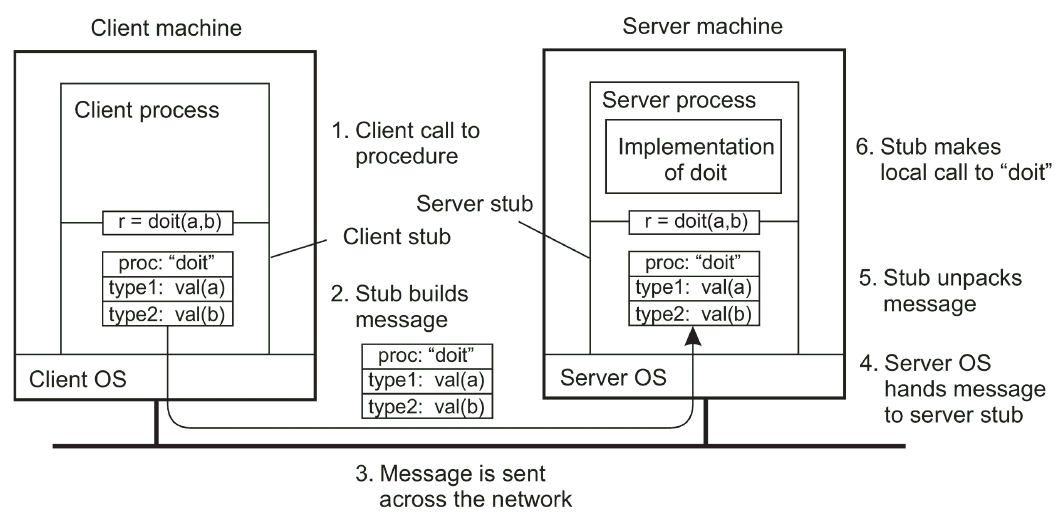
\includegraphics[scale=0.50]{img/how.png}
			\caption{Funzionamento RPC}
		\end{figure}
		Una chiamata a procedura remota deve essere \textbf{trasparente} rispetto al chiamante, per farlo viene creato uno stub locale della funzione che si trova in macchina remota. Lo stub, sia sul server che sul client implementa serializzazione e invio dei parametri e del risultato.  
		Di seguito si elencano i passi necessari ad una chiamata a procedura remota:
		\begin{enumerate}
			\item la procedura del client chiama il proprio stub;
			\item lo stub costruisce il messaggio ed effettua una chiamata al proprio OS;
			\item l'OS del client invia il messaggio all'OS remoto;
			\item l'OS remoto invia il messaggio allo stub del server;
			\item lo stub del server decomprime i parametri e chiama la procedura locale sul server;
			\item si esegue la computazione e si invia i risultati allo stub; 
			\item lo stub del server comprime i risultati e li invia al proprio OS;
			\item si invia il messaggio all'OS del client che lo passa allo stub del client;
			\item lo stub decomprime il risultato della computazione e lo passa al client
		\end{enumerate}
		
		\subsubsection{Passaggio di parametri}
			L'operazione di impacchettare parametri all'interno di un messaggio è chiamata \textbf{marhaling}, il messaggio conterrà i parametri stessi e le informazioni necessarie al destinatario. Il principale problema è il seguente: \textbf{client e server potrebbero adottare diverse rappresentazioni per i dati} (esempio diverse little endian big endian). Nel caso di utilizzo di HTTP come protocollo di trasporto il formato xml può essere utilizzato come formato comune per il passaggio dei parametri.
			\begin{figure}[h!]
				\centering
				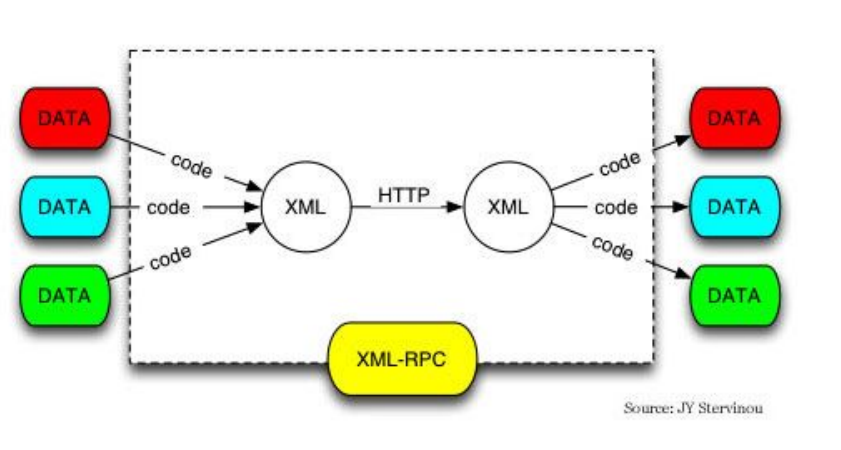
\includegraphics[scale=0.50]{img/xml.png}
				\caption{Xml }
			\end{figure}
		
			\textbf{Un problema} ulteriore risiede nel \textbf{passaggio dei puntatori e riferimenti}. Infatti, questi avranno senso solo se riferiti allo spazio di indirizzi locale del chiamante. Una possibile soluzione è quella di sostituire la \textbf{chiamata per riferimento} con un \textbf{copia/ripristina}. L'idea è quella di effettuare una copia dell'array da passare ed allegarla al messaggio destinato al server. L'array è conservato in un buffer nello stub del server ed inviato nuovamente al client una volta effettuata la chiamata remota (se richiesto). Nonostante i linguaggi offrano supporto automatico al \textbf{(un)marshaling}, quest'ultimo introduce un'\textbf{overhead} nella comunicazione, soprattutto in caso di grosse strutture dati come alberi e grafi.
			
			\begin{figure}[h!]
				\centering
				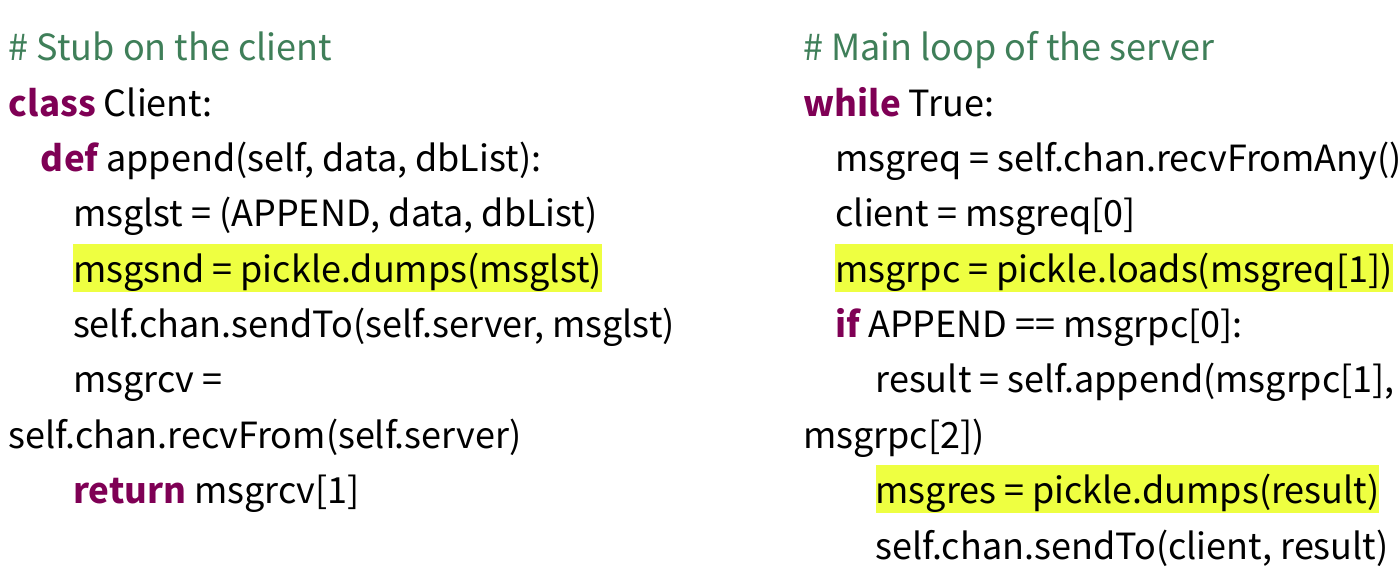
\includegraphics[scale=0.25]{img/rpccode.png}
				\caption{Marshaling in Java  }
			\end{figure}   
		
			Il problema non si presenta qualora i riferimenti siano \textbf{globali}, ovvero quando hanno un significato sia per il server sia per il client. \newline
			In generale, nel contesto di un sistema basato sugli oggetti sono definite due tipologie di oggetti:
			\begin{itemize}
				\item \textbf{Locali}: copiati e trasmessi nella loro interezza;
				\item \textbf{Remoti}: solo lo stub è copiato e trasmesso. 
			\end{itemize}
			In Java oggetti remoti o locali hanno tipi diversi (i remoti implementano l'interfaccia Remote).
			\begin{figure}[h!]
				\centering
				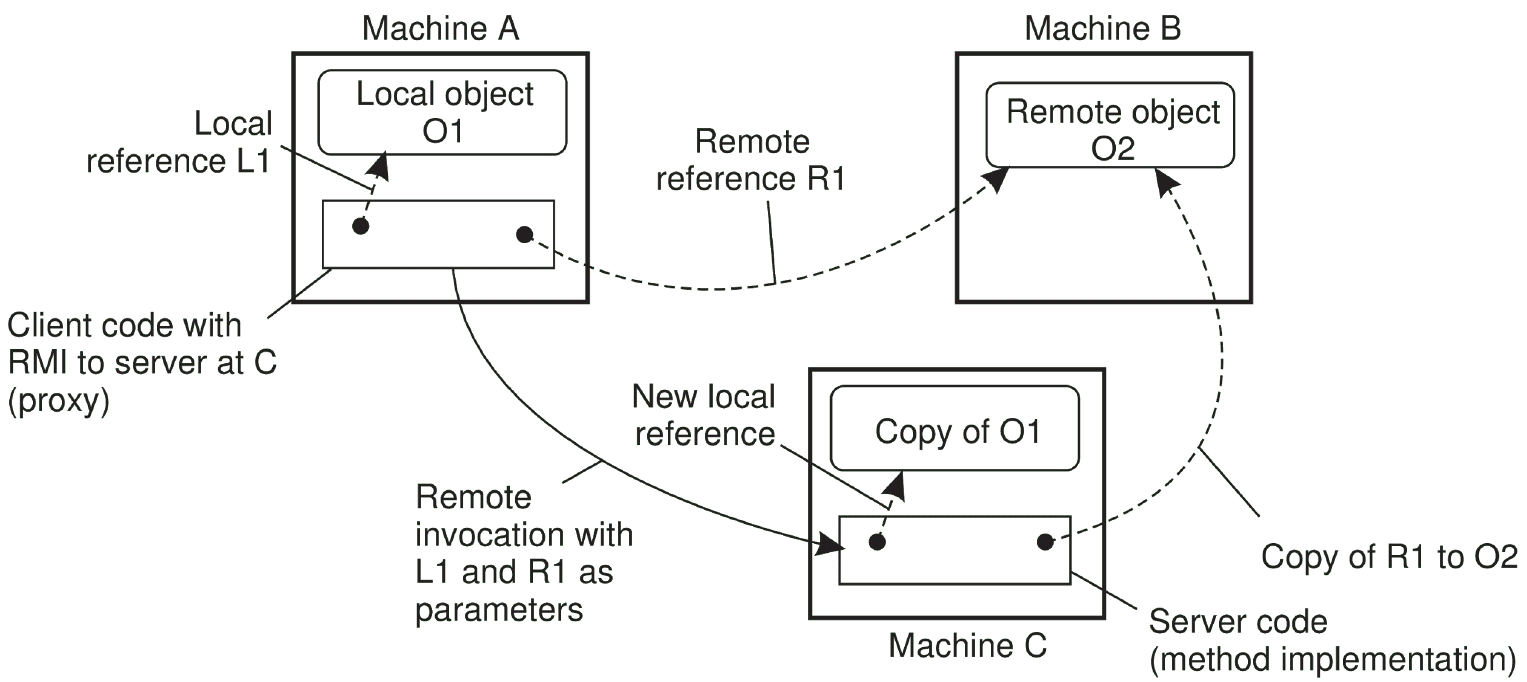
\includegraphics[scale=0.25]{img/remotelocal.png}
				\caption{Oggetti remoti e locali  }
			\end{figure}
		
		\subsubsection{Implementare RPC}
			Ci sono due modi attraverso il quale il meccanismo RPC può essere fornito allo sviluppatore:
			\begin{itemize}
				\item \textbf{Framework o libreria}: il programmatore deve specificare cosa è esportato in remoto fornendo di fatto un'\textbf{interfaccia del servizio}, che contiene tutte le procedure che possono essere chiamate dal client. I framework hanno il pregio di essere \textbf{indipendenti dal linguaggio}. Per questo è norma utilizzare un \textbf{Interface Definition Language (IDL)} che, una volta compilato, genere gli stub per client e server nel linguaggio desiderato. Di contro non abbiamo trasparenza totale per il programmatore che dunque è consapevole di trovarsi nel contesto di una chiamata a procedura remota (deve specificare egli stesso gli oggetti remoti). Alcuni esempi di framework: \textbf{Corba, GRPC, Apache Thrift}.     
				\item \textbf{Costrutti all'interno del linguaggio}: è lo stesso linguaggio a definire i costrutti necessari ad una RPC. In questo caso è il \textbf{compilatore a generare gli stub} per client e server. In questo modo si ottiene \textbf{trasparenza} per il programmatore, tuttavia client e server devono essere \textbf{implementati nello stesso linguaggio} (Es: \textbf{Java RMI}).
			\end{itemize}
		
		\subsubsection{RPC Asincrono}
			\begin{figure}[h!]
				\centering
				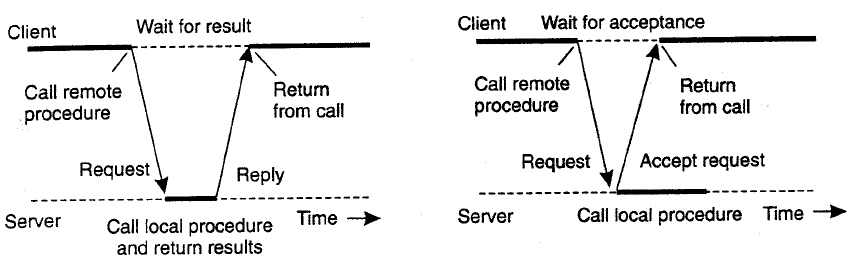
\includegraphics[scale=0.45]{img/async.png}
				\caption{RPC tradizionale e asincrona }
			\end{figure}
			A differenza del paradigma tradizionale nel quale il client attende la risposta del server bloccando la sua esecuzione, il server invia un ACK al client una volta ricevuta la richiesta. L'ACK viene inviato al client per notificare che la sua richiesta sarà processata, nel frattempo il client può eseguire ulteriori operazioni evitando di sospendere la sua esecuzione. Il Server utilizza una funzione detta di \textbf{Callback} per consegnare il risultato al Client.
			\begin{figure}[h!]
				\centering
				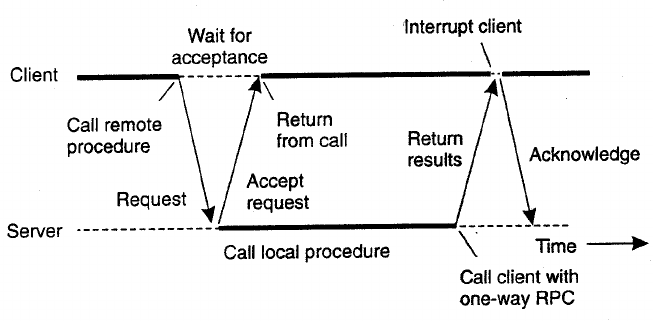
\includegraphics[scale=0.40]{img/callback.png}
				\caption{Callback }
			\end{figure}
			L'asincronicità della comunicazione permette l'implementazione di un protocollo \textbf{Multicast RPC} inviando richieste in parallelo a server diversi che dunque processano indipendentemente l'uno dall'altro. Si può definire questo protocollo nell'ottica di accettare il risultato più veloce scartando dunque gli altri, oppure per la realizzazione di una computazione distribuita, combinando i risultati ricevuti.
			
		\subsubsection{Binding}
			In applicazioni reali abbiamo bisogno di una fase preliminare chiamata \textbf{binding} che permette al client di avere un riferimento al server. Necessario per il client risulta l'utilizzo di un \textbf{registro} al cui interno sono salvate coppie (nome, indirizzo) di uno o più server. Si utilizza tale riferimento per la comunicazione.
			\begin{figure}[h!]
				\centering
				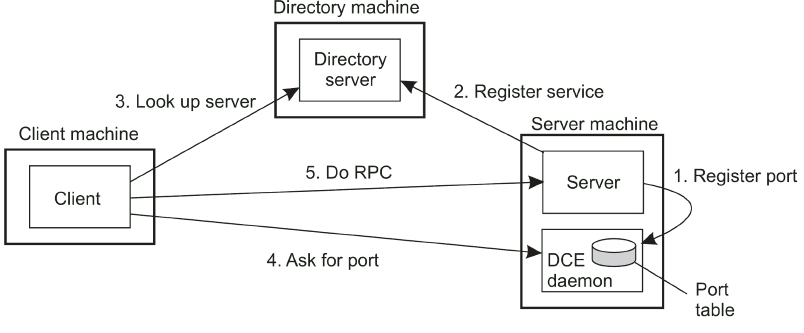
\includegraphics[scale=0.45]{img/bind.png}
				\caption{Binding }
			\end{figure}
		
	\subsection{Message Oriented Middleware}
		Questo modello di comunicazione prevede lo scambio di messaggi tra le entità partecipant. Grazie allo scambio di messaggi possiamo definire un modello nel quale, mittente e destinatario \textbf{non devono essere attivi durante lo scambio dei messaggi}. Questo è possibile grazie al Middleware che mette a disposizione buffer temporanei per i messaggi scambiati. Ogni applicazione ha a disposizione una coda locale che contiene i messaggi inviati e ricevuti e che può eventualmente essere condivisa tra più applicativi.
		\begin{figure}[h!]
			\centering
			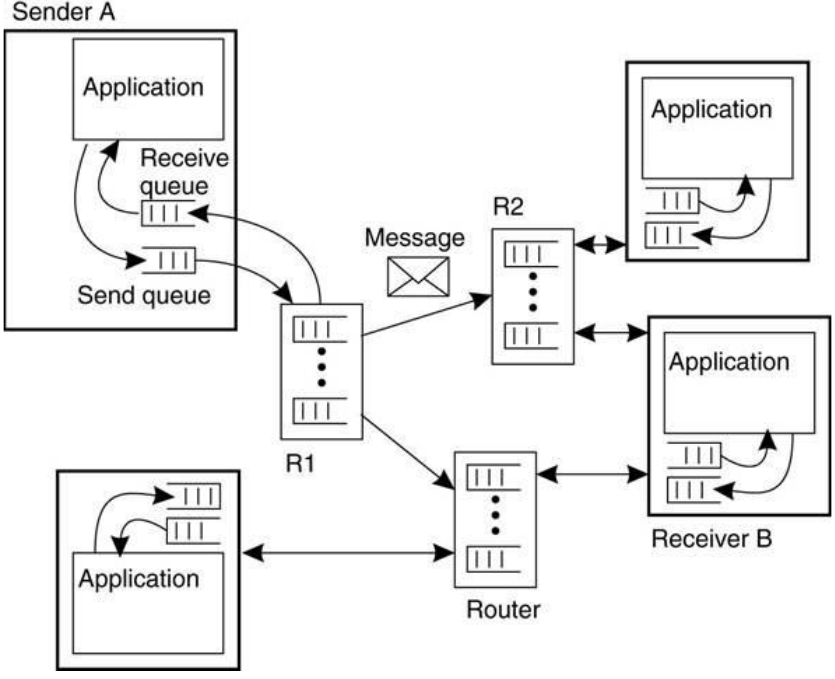
\includegraphics[scale=0.30]{img/queque.png}
			\caption{Code }
		\end{figure} 
		Il modello di comunicazione definito ha le seguenti proprietà:
		\begin{itemize}
			\item La comunicazione avviene semplicemente inserendo e rimuovendo messaggi dalla coda, un messaggio ovviamente rimane nella coda fino a che non è esplicitamente rimosso;
			\item La comunicazione è \textbf{loosely coupled}, cioò significa che il ricevente non deve essere necessariamente in esecuzione.   
		\end{itemize}
		Di seguito sono elencate le primitive concettuali che un message oriented middleware deve esporre:
		\begin{itemize}
			\item \textbf{Put}: inserisce un messaggio nella coda;
			\item \textbf{Get}: rimuove il primo messaggio dalla coda (blocking);
			\item \textbf{Poll}: rimuove il primo messaggio dalla coda (non-blocking);
			\item \textbf{Notify}: informa che un messaggio è arrivato nella coda.	
		\end{itemize}
		\newpage
		
		\subsubsection{Queue Manager}
			Il queue manager gestisce i messaggi inviati o ricevuti da un'applicazione nella sua coda (ad ogni applicazione è associata una coda e un relativo manager). Può essere implementato come una libreria collegata all'applicazione o come un \textbf{processo separato}. \textit{Nel secondo caso il sistema supporterà la comunicazione asincrona persistente}.
			\begin{figure}[h!]
				\centering
				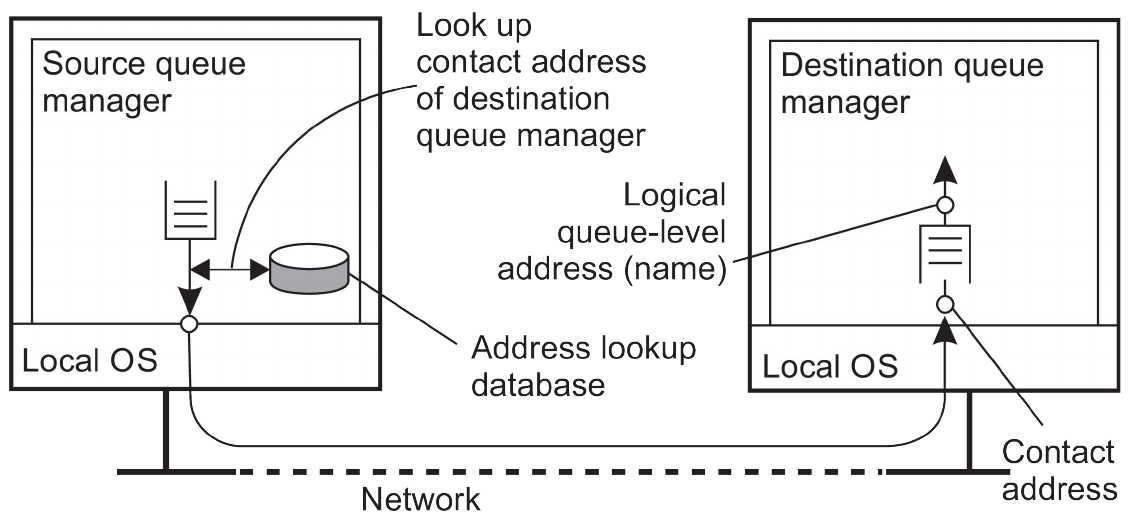
\includegraphics[scale=0.30]{img/mana.png}
				\caption{Queue Manager }
			\end{figure}
			In definitiva questi processi operano come \textbf{router} o \textbf{relay} inoltrando i messaggi ricevuti ad altri queue manager. In questo modo il sistema di quequing può costituire \textbf{un livello applicazione a se stante (Overlay network )} (un'astrazione), basato su una rete di computer esistente.
			\begin{figure}[h!]
				\centering
				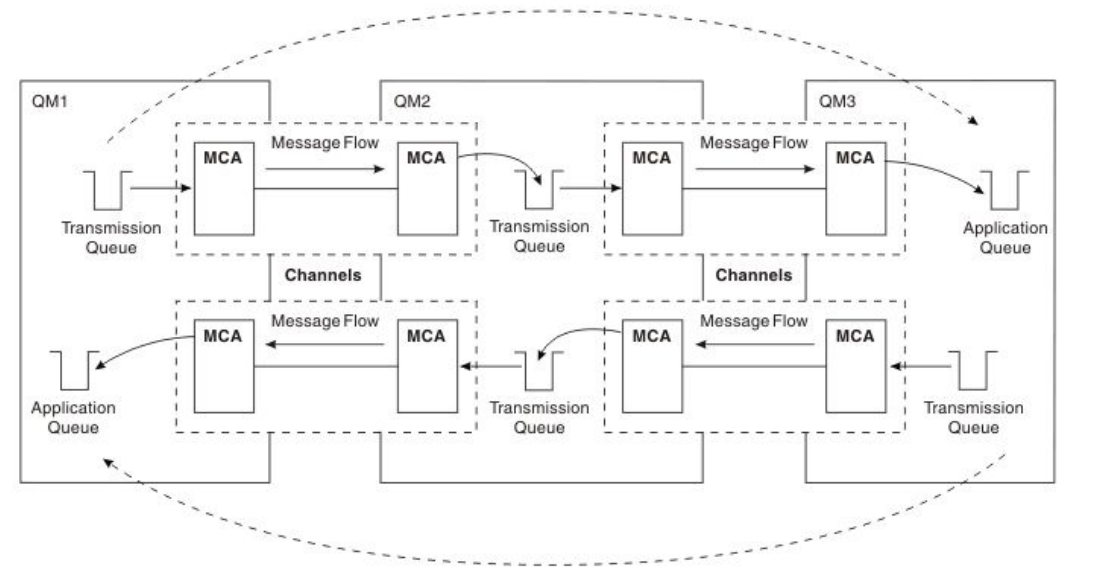
\includegraphics[scale=0.40]{img/overlay.png}
				\caption{Overlay network }
			\end{figure}
			Questa overlay network deve essere collegata e per farlo ogni entità deve essere a conoscenza degli indirizzi fisici associati ai nomi delle macchine partecipanti la rete e quindi delle loro rispettive code. Questo approccio \textbf{non risulta scalabile} e nel contesto di reti di grosse dimensioni porta ad evidenti \textbf{problemi gestionali}. Possiamo migliorare il modello di comunicazione delegando ai router la responsabilità di tenere traccia della topologia di rete e di aggiornare i binding (nome, indirizzo), mentre le altre entità partecipanti possiedono dei riferimenti statici al/ai router più vicino.
			
		\subsubsection{Eterogeneità: Message Brokers}
			I sistemi distribuiti possono essere eterogenei rispetto ai linguaggi utilizzati per realizzare le singole entità partecipanti. In questi casi è difficile definire un protocollo condiviso poichè è assente alla base un'accordo sul formato dei dati messaggi scambiati.\\
			Un \textbf{Message Broker} si comporta come un getway: si occupa di convertire i messaggi ricevuti in un formato consono a quello del ricevente. Nella pratica un message broker usa un repository di regole e programmi che permettono la conversione di un messaggio T1 in uno T2.
			Esempi di message brokers: 
			
	\subsection{Java RMI}
		Java RMI (\textbf{Remote Method Invocation}) è un framework che permette di implementare il modello RPC nel constesto di un sistema distribuito.
		\begin{figure}[h!]
			\centering
			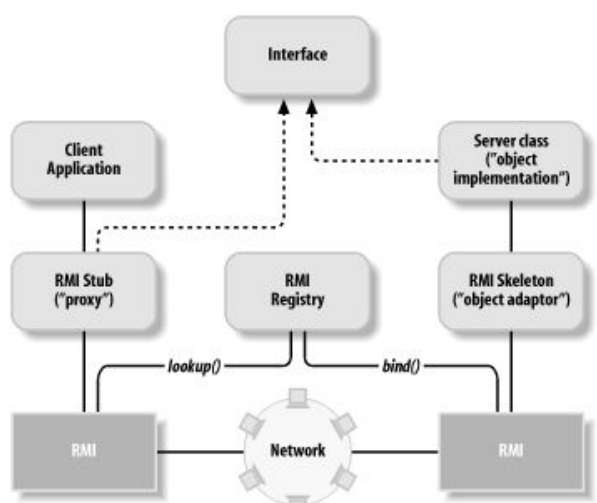
\includegraphics[scale=0.40]{img/rmi.png}
			\caption{Architettura di RMI}
		\end{figure}
		Il modello presenta 4 entità principali:
		\begin{itemize}
			\item \textbf{Interfaccia}: utilizzata per definire la risorsa remota;
			\item \textbf{Server}: implementa la risorsa remota (che sarà richiesta dal client);
			\item \textbf{Client}: richiede al server la risorsa remota.
			\item \textbf{Registro}: si occupa di gestire l'accesso alla risorsa remota.
		\end{itemize}
		Il \textbf{Registro}: è un servizio di \textbf{naming} che mappa i nomi simbolici degli oggetti remoti al loro stub. Il Server può registrare un oggetto remoto nel registro scrivendone il nome e l'indirizzo al quale è reperibile. Il client cerca l'oggetto remoto all'interno del registro.\\
		L'\textbf{interfaccia} specifica un contratto, ovvero le firme dei metodi che si possono invocare sull'oggetto remoto e che dunque ne regolano le modalità di utilizzo. \textbf{Per ogni oggetto} che vogliamo rendere accessibile attraverso la rete dobbiamo definire un'interfaccia che estenda l'interfaccia remota \textit{\textbf{java.rmi.remote}}. Le interfacce così definite dal server devono essere note anche al client in modo tale che egli possa operare sugli oggetti ricevuti dal server senza incorrere in errori di tipo. L'interfaccia remota serve solo ad indicare la possibilità di reperire gli oggetti che estendono tale interfaccia in remoto.\\
		Vediamo quali sono i passi per implementare un \textbf{RMI server}:
		\begin{enumerate}
			\item Implementare la classe remota definendo costruttore e metodi remoti (estendiamo la classe \textit{\textbf{java.rmi.server.UnicastRemoteObject }} e ne chiamiamo il costruttore per esportare l'oggetto);
			\item Creare un'istanza dell'oggetto remoto;
			\item Registrare tale oggetto remoto all'interno del registro. Per fare questo dobbiamo scegliere un identificativo unico (una stringa) per l'oggetto, che deve essere noto anche al client. Una volta ottenuto un riferimento al registry creiamo un binding tra quel nome e l'istanza dell'oggetto relativa. La classe \textit{\textbf{LocateRegistry}} permette di ottenere il riferimento al registro remoto o di crearne uno in ascolto sulla porta desiderata sullo stesso host del server (\textbf{\textit{createRegistry(int port), getRegistry(String host, int port )}}). 
		\end{enumerate}
		Per quanto riguarda il client i passi per l'implementazione sono i seguenti:
		\begin{enumerate}
			\item Localizzare il registro (stessi metodi della classe \textbf{LocateRegistry} indicati per il server);
			\item Utilizzare un nome simbolico per cercare l'oggetto remoto all'interno del registro;
			\item utilizzare l'oggetto remoto chiamandone i metodi. 
		\end{enumerate}
		Possiamo utilizzare RMI per implementare una comunicazione \textbf{sincrona} (il client aspetta fino al termine dell'invocazione remota). Possiamo ottenere una comunicazione \textbf{asincrona} utilizzando le \textbf{callback} il client invoca un oggetto remoto e passa la callback al server, utilizzata da quest'ultimo per ottenere  
		
	
		
		 
		
		
		  
			
			
			 
			 
	
		
		
		    
			
			 
			
			
			
		
		
			 
		
			 
			
			
			 
			
		
		
		
				
			
				
				
			
		
		
		
		
		
		
		
		
		
		
		
		
		
		
		
		
		
		
		
		
		
		
		
		
		
		
		
		

\end{document}